\documentclass[twocolumn,a4paper,10pt]{article}
\usepackage[utf8]{inputenc}
\usepackage[T1]{fontenc}
\usepackage{lmodern}
% babel português indisponível nesta instalação do TeX Live; nomes definidos manualmente
\renewcommand{\figurename}{Figura}
\AtBeginDocument{\renewcommand{\refname}{Referências}}
\usepackage[margin=1.8cm,top=2cm,bottom=1.8cm]{geometry}
\usepackage{amsmath}
\usepackage{booktabs}
\usepackage{graphicx}
\graphicspath{{figures/}}
\usepackage[font=small,skip=3pt]{caption}
\usepackage{tikz}
\usetikzlibrary{positioning, calc}
\usepackage{microtype}
\usepackage{titlesec}
\usepackage[colorlinks=true,linkcolor=black,citecolor=black,urlcolor=blue!50!black]{hyperref}

\setlength{\columnsep}{0.7cm}
\setlength{\parskip}{1pt}
\setlength{\textfloatsep}{8pt}
\setlength{\dbltextfloatsep}{9pt}
\titlespacing*{\section}{0pt}{6pt}{3pt}
\titleformat{\section}{\normalfont\large\bfseries}{\thesection}{0.6em}{}

\title{\vspace{-1.2cm}\Large\textbf{Síntese de Fala em Português com Tacotron2-VAE:\\ Estilo Copiado de um Áudio de Referência}}
\author{\normalsize Beatriz Nunes \quad Herivelton Siqueira \quad Richard Viana\\[2pt]
\small Machine Learning II --- IMPA Tech\\
\small Professores: Francisco Ganacim e Daniel Silveira Yukimura Lopez}
\date{\small Versão revisada --- novembro de 2026}

\begin{document}

\twocolumn[
\maketitle
\vspace{-0.9cm}
\begin{center}
\begin{minipage}{0.92\textwidth}
\small\textbf{Resumo ---} Implementamos um sistema de síntese de fala baseado no Tacotron~2 com um \textit{Variational Autoencoder} (VAE) que resume um áudio de referência em um vetor de estilo. Esta versão substitui a anterior, cujo resultado central (``atenção espectral interpretável'') vinha de um erro de código e não era válido. Corrigimos o erro, passamos a treinar a partir de um Tacotron~2 pré-treinado e conferimos todo áudio gerado por reconhecimento de fala. A taxa de palavras erradas caiu de 68\% para 2,2\% em inglês e de ininteligível para 10,5\% em português. Com o corpus emocional VERBO, a fala gerada copia a voz e o tom da referência, ao custo de inteligibilidade; um controle de intensidade do estilo recupera a inteligibilidade (9\% de erro) mantendo parte da emoção. Página do projeto: \url{https://rick0110.github.io/ml2_final_project}.
\end{minipage}
\end{center}
\vspace{0.3cm}
]

\section{Introdução}
Sistemas de síntese de fala produzem fala inteligível, mas com entonação fixa. O Tacotron2-VAE \cite{hsu,zhang} comprime um \textbf{áudio de referência} em um vetor latente $z$ que guarda o que o texto não determina (tom, velocidade, voz) e condiciona a síntese: o texto diz o que falar, a referência diz como. Nosso objetivo é ter esse sistema funcionando em português, como primeira peça de um sistema de dublagem.

\section{Revisão da versão anterior}
A versão anterior deste relatório propunha um \textit{pooling} por atenção no \textit{reference encoder} e interpretava seus pesos como bandas do espectro. A revisão do código mostrou três problemas. (i)~O mel de formato $(B, 80, T)$ era reorganizado com \texttt{view} sem transpor os eixos: tempo e frequência ficavam misturados e a posição dos blocos mudava com o \textit{padding} do lote. As ``bandas'' eram efeito desse erro. (ii)~A comparação com o \textit{baseline} usava treinos de 11,2 mil e 35,5 mil iterações, e não sustentava a conclusão sobre o colapso do latente. (iii)~Os áudios eram pouco inteligíveis: transcritos pelo Whisper \cite{whisper}, os 26 áudios em inglês tinham em média 68\% das palavras erradas e os dois em português não eram reconhecidos. Uma \texttt{LayerNorm} extra na atenção do decoder ainda impedia o uso de pesos pré-treinados. Todos os resultados abaixo são da versão corrigida.

\section{Arquitetura}
O sistema (Fig.~\ref{fig:pipeline}) segue o Tacotron~2 \cite{shen,nvidiataco}: um \textit{encoder} de texto (embedding + 3 Conv1d + BiLSTM), uma atenção sensível à localização, um decoder autoregressivo que prevê o mel quadro a quadro e o sinal de parada, e o vocoder \textbf{HiFi-GAN} universal \cite{hifigan}, pré-treinado e congelado. O inglês entra como caracteres e o português como fonemas IPA; os dois conjuntos ficam na mesma tabela de 199 símbolos, o que permite ajustar para o português um modelo treinado em inglês.

O \textit{reference encoder} \cite{skerry} aplica 6 convoluções 2D de \textit{stride}~2 ao mel de referência e uma GRU sobre os $T/64$ blocos de tempo resultantes ($\sim$0,74\,s cada). Os estados $h_t$ são resumidos por atenção, $e=\sum_t \alpha_t h_t$ com $\alpha=\mathrm{softmax}(w^\top h_t+b)$, com peso zero nos blocos de \textit{padding}. O resumo é projetado em $(\mu,\sigma)$; amostra-se $z$ de 32 dimensões, convertido em um vetor de estilo somado a todas as posições da saída do \textit{encoder}. Não comparamos esse resumo com o último estado da GRU, e por isso não afirmamos que seja melhor.

\begin{figure*}[t]
    \centering
    \resizebox{0.88\textwidth}{!}{%
    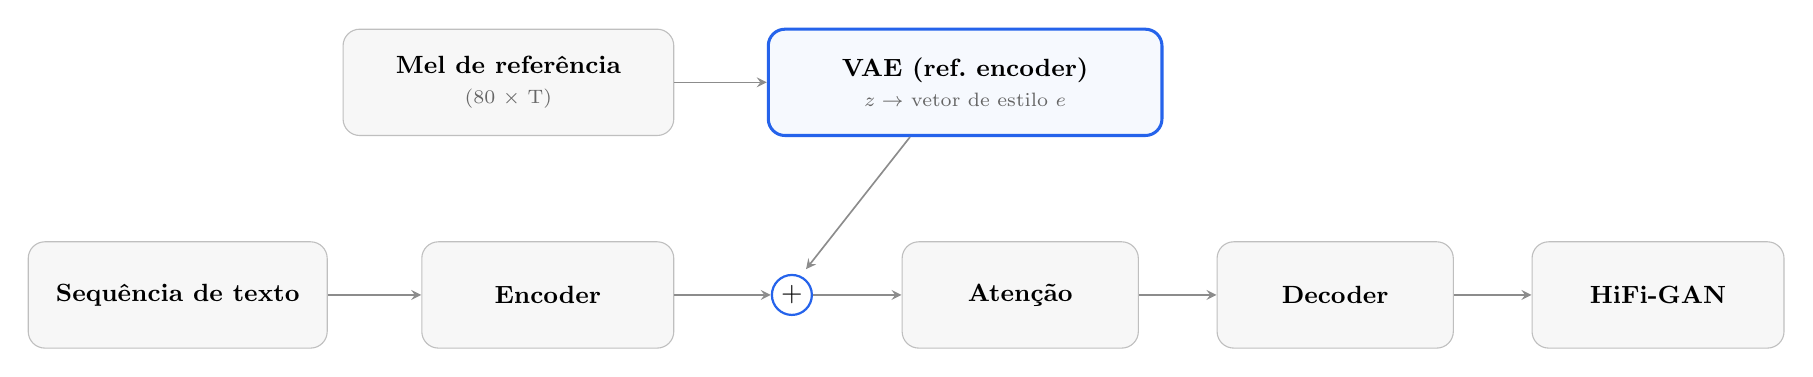
\begin{tikzpicture}[
        box/.style={rectangle, draw=black!25, rounded corners=6pt, fill=black!3, minimum height=1.35cm, text centered, font=\small\bfseries, align=center, inner xsep=10pt},
        boxhl/.style={box, draw=refblue, line width=1.1pt, fill=refblue!4},
        arrow/.style={->, >=stealth, semithick, draw=black!45}
    ]
    \definecolor{refblue}{RGB}{37,99,235}
    % linha superior (ramo de estilo)
    \node[box, minimum width=4.2cm] (mel) at (6.6,0) {Mel de referência\\{\scriptsize\mdseries\color{black!60}(80 $\times$ T)}};
    \node[boxhl, minimum width=5cm] (vae) at (12.4,0) {VAE (ref.\ encoder)\\{\scriptsize\mdseries\color{black!60}$z \rightarrow$ vetor de estilo $e$}};
    % linha inferior (pipeline principal)
    \node[box, minimum width=3.7cm] (texto) at (2.4,-2.7) {Sequência de texto};
    \node[box, minimum width=3.2cm] (encoder) at (7.1,-2.7) {Encoder};
    \node[circle, draw=refblue, thick, fill=white, inner sep=1.5pt, font=\normalsize] (soma) at (10.2,-2.7) {$+$};
    \node[box, minimum width=3cm] (atencao) at (13.1,-2.7) {Atenção};
    \node[box, minimum width=3cm] (decoder) at (17.1,-2.7) {Decoder};
    \node[box, minimum width=3.2cm] (waveglow) at (21.2,-2.7) {HiFi-GAN};
    % setas
    \draw[arrow] (mel) -- (vae);
    \draw[arrow] ([xshift=-0.7cm]vae.south) -- ($(soma.north)+(0.18,0.06)$);
    \draw[arrow] (texto) -- (encoder);
    \draw[arrow] (encoder) -- (soma);
    \draw[arrow] (soma) -- (atencao);
    \draw[arrow] (atencao) -- (decoder);
    \draw[arrow] (decoder) -- (waveglow);
    \end{tikzpicture}%
    }
    \caption{\small Arquitetura do sistema: o VAE comprime o Mel de referência no vetor de estilo $e$, somado ($+$) a cada posição da memória do \textit{encoder}; atenção e decoder geram o Mel-espectrograma, convertido em áudio pelo HiFi-GAN.}
    \label{fig:pipeline}
\end{figure*}

\section{Treinamento}
A perda combina quatro termos:
\begin{equation*}
\mathcal{L} = \mathcal{L}_{\text{mel}} + \mathcal{L}_{\text{gate}} + \beta(\text{passo})\,\mathcal{L}_{\text{KL}} + \lambda\,\mathcal{L}_{\text{GA}},
\end{equation*}
com MSE do mel, entropia cruzada do sinal de parada, KL com \textit{free bits} de 0,5 e $\beta$ cíclico (0 a 0,2), e atenção guiada \cite{tachibana}. Treinar do zero não cabia no orçamento e era a causa provável dos alinhamentos ruins; por isso o treino é feito em etapas, cada uma partindo da anterior (Tab.~\ref{tab:etapas}), em uma GPU L4, com Adam ($lr=10^{-4}$) e 28,9\,M de parâmetros.

\begin{table}[h]
\centering\small
\begin{tabular}{@{}llr@{}}
\toprule
Etapa & Dados & Passos\\
\midrule
Inglês & LJSpeech, 23,7\,h & 2.500\\
Português & TTS-Portuguese \cite{ttspt}, 3,8\,h & 4.000\\
Emoção & TTS-Port. + VERBO \cite{verbo} & 1.500\\
\bottomrule
\end{tabular}
\caption{Etapas de treino. A primeira parte do Tacotron~2 pré-treinado da NVIDIA; cada uma das seguintes parte da anterior. O VERBO tem 1.167 falas de 12 locutores em 7 emoções, com apenas 14 frases distintas.}
\label{tab:etapas}
\end{table}

\begin{figure}[t]
    \centering
    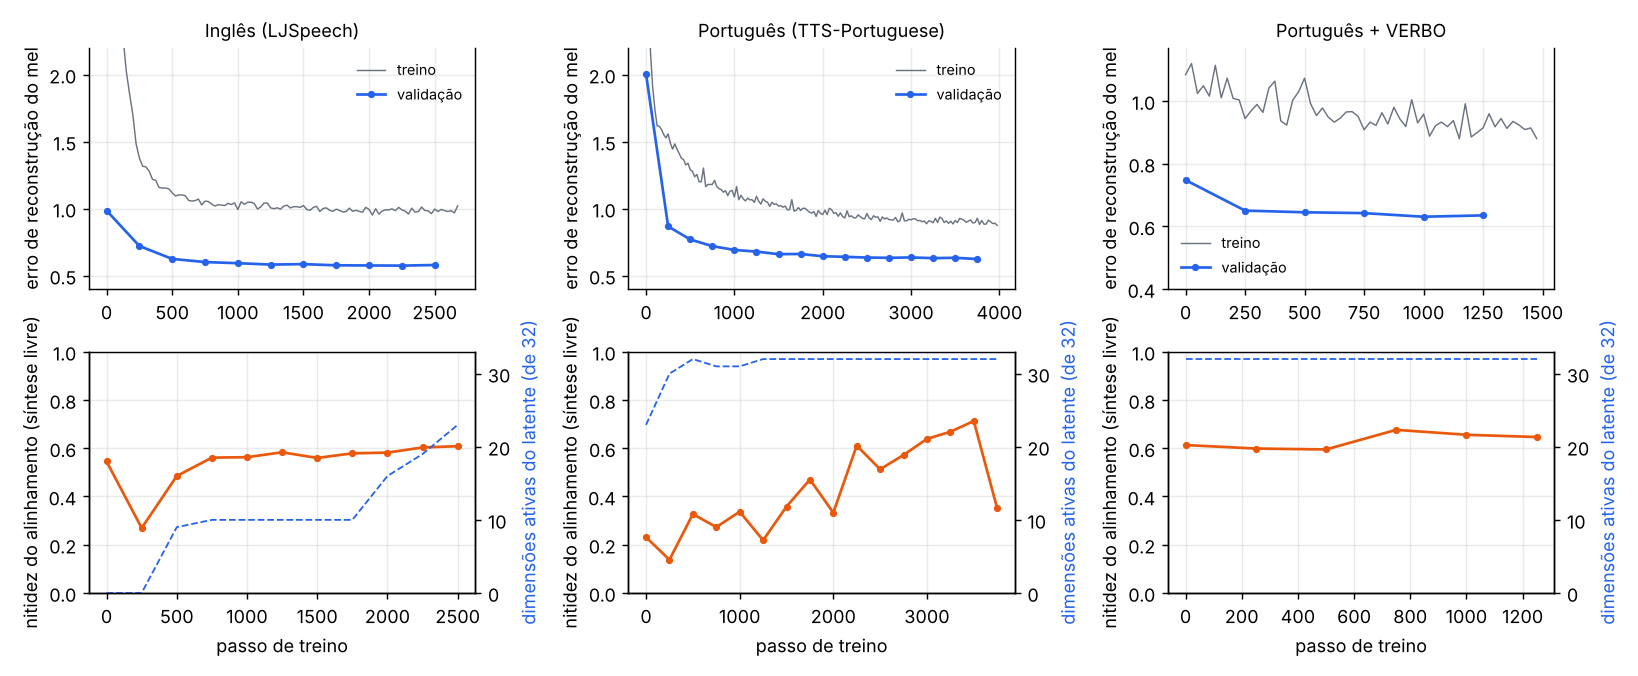
\includegraphics[width=\columnwidth]{fig_retreino_curvas}
    \caption{Em cima: erro de reconstrução do mel (treino em cinza, validação em azul; o treino é maior porque metade dos quadros de entrada do decoder é descartada). Embaixo: nitidez do alinhamento na síntese livre (laranja) e dimensões ativas do latente (tracejado).}
    \label{fig:curvas}
\end{figure}

\section{Avaliação}
Para cada modelo sintetizamos 6 frases fora do treino com várias referências. Cada áudio é transcrito pelo Whisper \textit{small} e comparado com o texto pedido (taxa de palavras erradas, WER). Medimos também se o decoder para sozinho, o tom médio (F0) e a velocidade (caracteres por segundo) do áudio gerado e da referência.

\begin{figure}[t]
    \centering
    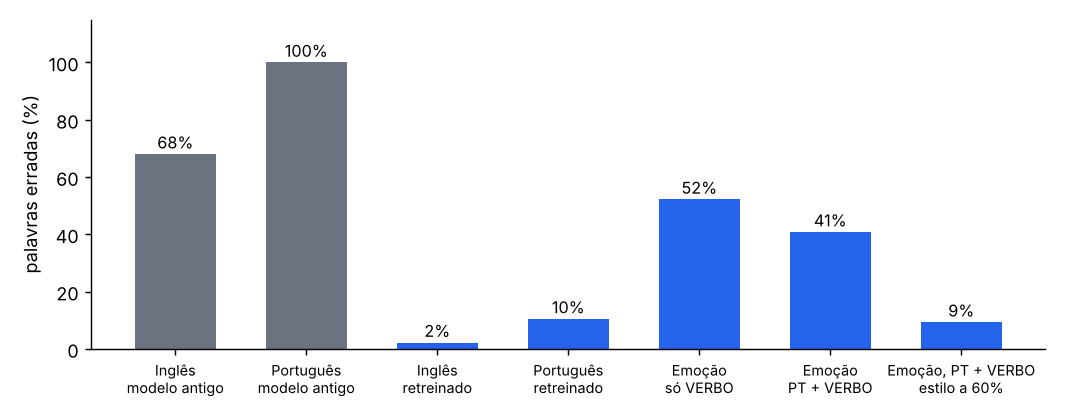
\includegraphics[width=\columnwidth]{fig_retreino_wer}
    \caption{Palavras erradas na transcrição automática dos áudios gerados. Cinza: modelos anteriores. Azul: retreinados.}
    \label{fig:wer}
\end{figure}

\textbf{Inglês.} WER de 2,2\% em 18 áudios, todos terminando sozinhos; os três erros são a mesma palavra (``stone''). Tom e velocidade não acompanharam as referências: o LJSpeech é uma locutora com leitura uniforme, e há pouca variação de estilo a aprender.

\textbf{Português.} WER de 10,5\% em 18 áudios, todos terminando sozinhos (Fig.~\ref{fig:wer}). Os erros são trocas pontuais (``carrega''$\to$``cariga''). A velocidade da fala acompanha a referência: com referências de 9,1, 12,6 e 16,3 caracteres/s, a mesma frase saiu com 8,8, 11,9 e 12,7. As 32 dimensões do latente ficam ativas (Fig.~\ref{fig:curvas}).

\begin{figure}[t]
    \centering
    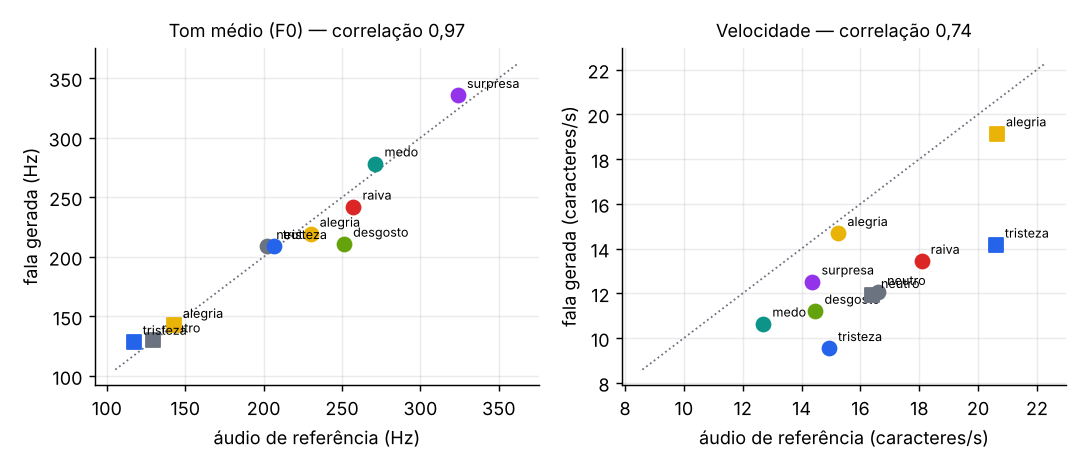
\includegraphics[width=\columnwidth]{fig_retreino_estilo_ptverbo_vae_v1}
    \caption{Modelo português + VERBO, estilo inteiro: tom e velocidade da fala gerada contra os da referência (círculos: locutora f1; quadrados: locutor m1).}
    \label{fig:estilo}
\end{figure}

\begin{figure}[t]
    \centering
    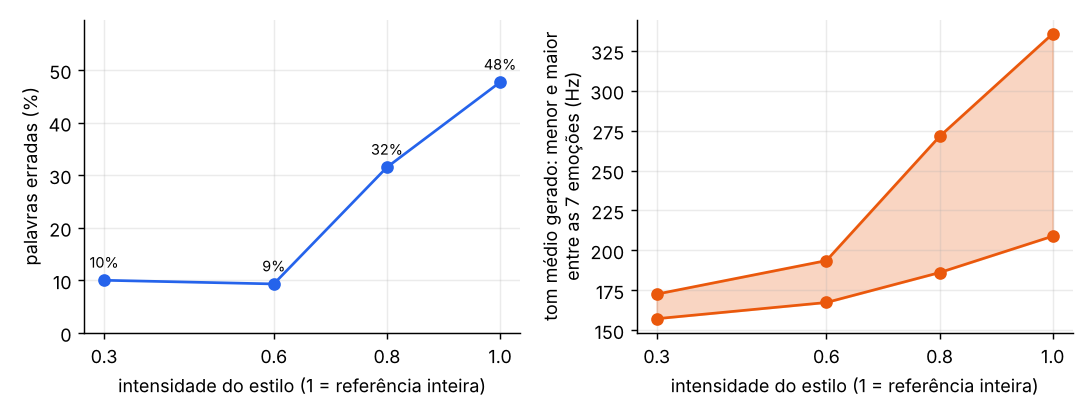
\includegraphics[width=\columnwidth]{fig_retreino_intensidade}
    \caption{Efeito da intensidade do estilo (7 emoções da locutora f1): palavras erradas e faixa do tom médio entre as emoções.}
    \label{fig:intensidade}
\end{figure}

\textbf{Emoção.} Usamos 10 referências do VERBO (7 emoções da locutora f1 e 3 do locutor m1). O modelo de português, sem ver o VERBO, mantém a própria voz (WER 19\%, sem relação entre o tom gerado e o da referência). Ajustado só no VERBO, o modelo copia voz e tom (correlação 0,96 entre o F0 gerado e o da referência), mas o WER sobe para 52\%: com 14 frases, ele desaprende a ler texto novo. Treinando com os dois corpora juntos, o tom continua seguindo a referência (correlação 0,97, Fig.~\ref{fig:estilo}) e o WER cai para 41\%, ainda alto.

\textbf{Intensidade do estilo.} O erro vem de sintetizar com vozes que o modelo só ouviu em 14 frases. Multiplicando o código latente da referência por um fator $a\in[0,1]$ antes da síntese, $z = a\,\mu_{\text{ref}}$, obtemos um controle contínuo (Fig.~\ref{fig:intensidade}): com $a=0{,}6$ o WER cai para 9\% e a velocidade ainda varia com a emoção (de 9,3 a 14,1 caracteres/s), mas o tom fica próximo do neutro. Emoção forte e fala clara não foram obtidas ao mesmo tempo; o limite está no corpus, não no modelo.

\section{Conclusão}
O resultado central da versão anterior era um erro e foi retirado. Com o código corrigido e o treino a partir de um modelo pré-treinado, o sistema fala inglês e português de forma inteligível e copia da referência a velocidade e, com dados de vários locutores e emoções, a voz e o tom. Com o VERBO, copiar a emoção por inteiro custa inteligibilidade, e o controle de intensidade do estilo permite escolher o ponto desse compromisso. Limitações: a avaliação usa poucas frases e mede só inteligibilidade, não naturalidade; o vetor de estilo é global e não varia ao longo da frase; o \textit{pooling} por atenção não foi comparado com a alternativa mais simples. Para a dublagem faltam o controle de duração das falas, o vídeo como entrada e a sincronia labial.

\begin{thebibliography}{99}\footnotesize\setlength{\itemsep}{1pt}\setlength{\parskip}{0pt}
\bibitem{hsu} Hsu, W.-N. et al. \textit{Hierarchical Generative Modeling for Controllable Speech Synthesis}. ICLR, 2019.
\bibitem{zhang} Zhang, Y.-J., Pan, S., He, L., Ling, Z.-H. \textit{Learning Latent Representations for Style Control and Transfer in End-to-End Speech Synthesis}. ICASSP, 2019. arXiv:1812.04342.
\bibitem{shen} Shen, J. et al. \textit{Natural TTS Synthesis by Conditioning WaveNet on Mel Spectrogram Predictions}. ICASSP, 2018. arXiv:1712.05884.
\bibitem{nvidiataco} NVIDIA. \textit{Tacotron 2} (implementação de referência). \url{https://github.com/NVIDIA/tacotron2}.
\bibitem{hifigan} Kong, J., Kim, J., Bae, J. \textit{HiFi-GAN: Generative Adversarial Networks for Efficient and High Fidelity Speech Synthesis}. NeurIPS, 2020.
\bibitem{skerry} Skerry-Ryan, R.J. et al. \textit{Towards End-to-End Prosody Transfer for Expressive Speech Synthesis with Tacotron}. ICML, 2018.
\bibitem{tachibana} Tachibana, H. et al. \textit{Efficiently Trainable Text-to-Speech System Based on Deep Convolutional Networks with Guided Attention}. 2017.
\bibitem{ttspt} Casanova, E. et al. \textit{TTS-Portuguese Corpus: a corpus for speech synthesis in Brazilian Portuguese}. Language Resources and Evaluation, 2022.
\bibitem{verbo} Torres Neto, J. R. et al. \textit{VERBO: Voice Emotion Recognition dataBase in Portuguese Language}. Journal of Computer Science, 2018.
\bibitem{whisper} Radford, A. et al. \textit{Robust Speech Recognition via Large-Scale Weak Supervision}. ICML, 2023.
\end{thebibliography}

\end{document}
